\documentclass[10pt,handout]{beamer}

\usetheme{Madrid}
\usecolortheme{default}

% Base packages
%\usepackage{helvet}
\usepackage{amsthm,graphicx,xcolor,natbib,booktabs,tabularx,mathtools,subcaption}
\usepackage{unicode-math,mathrsfs}
\usepackage{amsmath,amssymb}
\usepackage{tikz,pgfplots}
\usetikzlibrary{arrows.meta, positioning, quotes}

%\usepackage[cache=false]{minted}
%\renewcommand{\theFancyVerbLine}{\sffamily\textcolor[rgb]{0.5,0.5,1.0}{\scriptsize\oldstylenums{\arabic{FancyVerbLine}}}}
%\definecolor{bg}{rgb}{.95,.95,.95}

% Font settings
\renewcommand{\familydefault}{\sfdefault}

% TikZ libraries
\usetikzlibrary{calc,positioning,backgrounds,decorations.pathreplacing}
\pgfplotsset{compat=1.14}

% Colors
\definecolor{deepblue}{RGB}{42,39,155}
\definecolor{lightpink}{RGB}{255,240,240}
\definecolor{lightgreen}{RGB}{240,255,240}
\definecolor{lightyellow}{RGB}{255,255,240}
\definecolor{codegray}{RGB}{245,245,245}
\definecolor{codegreen}{rgb}{0,0.6,0}
\definecolor{codepurple}{rgb}{0.58,0,0.82}

% Beamer settings
\setbeamercolor{title}{fg=white,bg=deepblue}
\setbeamercolor{frametitle}{fg=white,bg=deepblue}
\setbeamercolor{section in head/foot}{fg=white,bg=deepblue}

\setbeamertemplate{footline}[text line]{%
  \parbox{\linewidth}{\vspace*{-8pt}
  %\hfill\href{https://github.com/chang-ye-tu/fin}{https://github.com/chang-ye-tu/fin}
    \hfill
   \insertframenumber~/ \inserttotalframenumber}}
\setbeamertemplate{navigation symbols}{}%[only frame symbol]

\definecolor{foo}{rgb}{.2,.2,.7}
\AtBeginSection[]{
  \begin{frame}
  \vfill
  \centering
  \begin{beamercolorbox}[sep=8pt,center,shadow=true,rounded=true]{section page}
    \usebeamerfont{title}%
    {\color{foo} \insertsectionhead}\par%
  \end{beamercolorbox}
  \vfill
  \end{frame}
}

% https://tex.stackexchange.com/questions/30423/bibliography-in-beamer
\setbeamertemplate{bibliography entry title}{}
\setbeamertemplate{bibliography entry location}{}
\setbeamertemplate{bibliography entry note}{}

\newcommand{\ds}{\displaystyle}
\newcommand{\ie}{\;\Longrightarrow\;}
\newcommand{\ifff}{\;\Longleftrightarrow\;}
\newcommand{\mi}{\mathrm{i}}
\DeclareMathOperator*{\dom}{dom}
\DeclareMathOperator*{\codom}{codom}
\DeclareMathOperator*{\ran}{ran}
\newcommand{\floor}[1]{\lfloor #1 \rfloor}
\newcommand{\ceil}[1]{\lceil #1 \rceil}
\newcommand{\Set}[2]{\big\{ \ #1\ \big|\ #2\ \big\}}
\newcommand{\pdiff}[2]{\frac{\partial\hfil#1\hfil}{\partial #2}}
\newcommand{\vx}{\symbfup{x}}
\newcommand{\vd}{\symbfup{d}}
\newcommand{\vg}{\symbfup{g}}
\newcommand{\vH}{\symbfup{H}}
\newcommand{\va}{\symbfup{a}}
\newcommand{\vb}{\symbfup{b}}
\newcommand{\vbb}{\symbfup{\beta}}
\newcommand{\vS}{\symbfup{S}}
\newcommand{\vR}{\symbfup{R}}
\newcommand{\vV}{\symbfup{V}}
\newcommand{\ve}{\symbfup{e}}
\newcommand{\vr}{\symbfup{r}}
\newcommand{\vZero}{\symbfup{0}}

\DeclareMathOperator\prb{{\sf P}}
\DeclareMathOperator\expc{{\sf E}}
\DeclareMathOperator\var{var}
\DeclareMathOperator\cov{cov}
\DeclareMathOperator\cor{cor}
\DeclareMathOperator*{\argmax}{\arg\!\max}
\DeclareMathOperator*{\argmin}{\arg\!\min}
\DeclareMathOperator*{\im}{Im}
\DeclareMathOperator*{\re}{Re}
\DeclareMathOperator*{\conv}{conv}
\DeclareMathOperator*{\proj}{proj}
\DeclareMathOperator*{\tr}{tr}
\DeclareMathOperator*{\diag}{diag}
\DeclareMathOperator*{\epi}{epi}
\DeclareMathOperator*{\dist}{dist}
\DeclareMathOperator*{\inte}{int}
\DeclareMathOperator*{\relint}{relint}

\theoremstyle{definition}
\newtheorem*{dfn}{Definition}
\newtheorem*{prp}{Property}
\newtheorem*{thm}{Theorem}
\newtheorem*{ex}{Example}
\newtheorem*{prob}{Problem}
\newtheorem*{sol}{Solution}
\newtheorem*{prf}{Proof}
\usepackage{nicefrac}

\newcommand\scalemath[2]{\scalebox{#1}{\mbox{\ensuremath{\displaystyle #2}}}}

\title{Options \& Derivatives}
\author{}
\date{}

\begin{document}

\begin{frame}
\titlepage
\end{frame}

%\subsection*{Outline}
%\begin{frame}
%  \tableofcontents
%\end{frame}

\begin{frame}{The One Period Model}
  \begin{itemize}
    \item time $t$: $t=0, 1$ 
    \item (deterministic) bond $B_t$: $\ds B_0 = 1,\;B_1 = 1 + R$
    \item (stochastic) stock $S_t$: $\ds S_0 = s > 0, \; S_1 = \begin{cases} s\cdot u & \text{with prob. } p_u\\ s\cdot d & \text{with prob. } p_d \end{cases} \equiv s\,Z:\;$ $u > d$, $p_u + p_d = 1$.
    \item The value $V_t^h$ of the portfolio $h=(x, y),\,x, y\in\mathbb{R}$ at time $t$: $\ds V_t^h = x\,B_t + y\,S_t$ --- $\ds V_0^h = x + y\,s,\; V_1^h = x(1 + R) + y\,s\,Z$
    \item Arbitrage portfolio $h$: $V_0^h=0$, $V_1^h>0$ with prob. $1$.
  \end{itemize}
  \begin{figure}[!htbp]
    \centering
    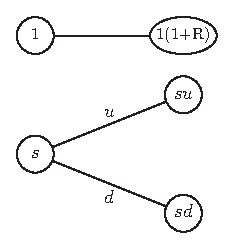
\includegraphics[scale=0.9,page=1]{fig/bjork.pdf}
    \caption{Asset Dynamics of One Period Model.}
    \label{fig:bn1}
  \end{figure}
\end{frame}

\begin{frame}{Portfolios and Arbitrage I}
  \begin{thm}
    The one period model is arbitrage free $\ifff$ $\ds u\geqslant 1+R \geqslant d$.
  \end{thm}
  \begin{prf}
    ($\Longrightarrow$)
    \begin{itemize}
      \item Suppose $u\geqslant 1+R \geqslant d$ does not hold, then $1 + R > u$ or $d > 1 + R$.
      \item If $1 + R > u$, then $s(1 + R) > s\,u$ and a priori $s(1+R) > s\,d$.
      \item Consider $h = (s, -1)$, then $V_0^h = s\cdot 1 + (-1)\cdot s = 0$, $V_1^h = s(1 + R) - s\cdot Z >0$, an arbitrage.
      \item If $d > 1 + R$, then $s\,d > s(1 + R)$ and a priori $s\,u > s(1 + R)$.
      \item Consider $h = (-s, 1)$, then $V_0^h = (-s)\cdot 1 + 1\cdot s = 0$, $V_1^h = -s(1 + R) + s\cdot Z > 0$, an arbitrage.
    \end{itemize}
  \end{prf}
\end{frame}
\begin{frame}{Portfolios and Arbitrage II}
  \begin{thm}
    The one period model is arbitrage free $\ifff$ $\ds u\geqslant 1+R \geqslant d$.
  \end{thm}
  \begin{prf}
    ($\Longleftarrow$)
    \begin{itemize}
      \item Arbitrage $h = (x, y)$: $V_0^h = 0$.
      \item $ x + s\cdot y = 0\ie x= -s\cdot y$. 
      \item $\ds V_1^h = \begin{cases}y\,s\big(u - (1 + R)\big),&\; Z=u \\ y\,s\big(d - (1 + R)\big),&\; Z=d\end{cases}$
      \item If $y > 0$: from $\ds V_1^h > 0$ $\ie$ $u > 1 + R$ and $d > 1 + R$; a contradiction.
      \item If $y < 0$: from $\ds V_1^h > 0$ $\ie$ $u < 1 + R$ and $d < 1 + R$; a contradiction.
    \end{itemize}
  \end{prf}
\end{frame}

%\begin{thm}
%  $\ds \text{ No arbitrage }\ifff u\geqslant 1+R \geqslant d$
%\end{thm}

\begin{frame}{Risk-Neutral / Martingale Measure and Probabilities}
  \begin{itemize}
    \item Observation: $u\geqslant 1+R \geqslant d$ $\ie$ $1 + R$ is a convex combination of $u$ and $d$  
    \item $\ds\exists\,q_u, q_d \geqslant 0,\,\,q_u+q_d = 1\;\text{ s.t. }\; 1 + R = q_u\cdot u + q_d\cdot d$
    \item Define a new probability measure $Q$ and the associated expectation $\expc^Q$ s.t. 
      \begin{align*}
        &Q(Z = u) = q_u,\quad Q(Z = d) = q_d \\
        &\frac{1}{1+R}\expc^Q S_1 = \frac{1}{1+R}(q_u\cdot s\,u + q_d\cdot s\,d) = \frac{1}{1+R}\cdot s(1+R) = s
      \end{align*}
  \end{itemize}
  \begin{dfn}
    \begin{itemize}
      \item \textbf{Risk-Neutral / Martingale Measure}: A measure $Q$ satisfies $\ds S_0 = \frac{1}{1+R}\expc^Q S_1$.
      \item \textbf{Martingale Probabilities}: $\ds q_u = \frac{(1+R)-d}{u-d}, \;q_d = \frac{u-(1+R)}{u-d}$
    \end{itemize}
  \end{dfn}
\end{frame}

\begin{frame}{Contingent Claims I}
  \begin{dfn}
    \begin{itemize}
      \item A \textbf{contingent claim} $X$ is of the form $X=\Phi(Z)$
      \item Stochastic $Z$ with \textbf{contract function} $\Phi(\cdot)$
      \item \textbf{Price} of $X$ at time $t$: $\Pi(t; X)$
    \end{itemize}
  \end{dfn}
  \begin{figure}[!htbp]
    \centering
    \includegraphics[scale=.9,page=2]{fig/bjork.pdf}
    \caption{The Contingent Claim.}
    \label{fig:bn2}
  \end{figure}
\end{frame}

\begin{frame}{Contingent Claims II}
  \begin{example}[European Call Option with Strike $K$]
    Assume $s\, u > K > s\, d$. At $t=1$, 
    \begin{itemize}
      \item Exercise the option if $S_1 > K$.
        \begin{itemize}
          \item Pay $K$ to get the stock and sell it at $s\,u$, thus making net profit $s\,u-K$.
        \end{itemize}
      \item Do nothing if $S_1 < K$.
    \end{itemize}
    \begin{align*}
      X = \begin{cases}s\,u - K, & Z=u \\ 0,  & Z=d\end{cases}, \quad\begin{cases}\Phi(u) = s\, u - K \\ \Phi(d) = 0\end{cases}
    \end{align*}
  \end{example}
  \begin{dfn}
    \begin{itemize}
      \item A contingent claim $X$ is said to be \textbf{reachable} if there exists a portfolio $h$ such that $V_1^h = X$ with probability 1; this portfolio $h$ is called a \textbf{hedging} or \textbf{replicating} portfolio. 
      \item If all claims can be replicated we say the market is \textbf{complete}.
    \end{itemize}
  \end{dfn}
\end{frame}

\begin{frame}{Contingent Claims III}
\begin{thm}[Pricing Principle]
  If a claim $X$ is reachable with replicating portfolio $h$, then the ``reasonable'' price of $X$ is given by $\ds\Pi(t; X) = V_t^h, \; t=0, 1.$
\end{thm}

\begin{thm}
  An arbitrage free one period model is complete.
\end{thm}

\begin{prf}
  Fixed any $\Phi(\cdot)$, show that $\exists\,h=(x, y)$ s.t.
  \begin{align*}
    V_1^h = \begin{cases}\Phi(u)\quad Z=u,\\ \Phi(d)\quad Z=d.\end{cases}\!\!\!\!\Longrightarrow x(1+R) + y\,s\,u = \Phi(u), \; x(1+R) + y\,s\,d = \Phi(d).
  \end{align*}
  Solve for $x, y$: $\ds x = \frac{1}{1+R}\,\frac{u\Phi(d)-d\,\Phi(u)}{u-d},\quad y = \frac{1}{s}\,\frac{\Phi(u)-\Phi(d)}{u-d}$.
\end{prf}
\end{frame}

\begin{frame}{Risk Neutral Valuation}
  \begin{itemize}
    \item From Pricing Principle ($\Pi(t; X) = V_t^h,\, t=0,1$)
      \begin{align*}
        \Pi(0; X) &= V_0^h = x + s\,y \\
                  &= \frac{1}{1+R}\cdot\frac{u\Phi(d)-d\,\Phi(u)}{u-d} + s\cdot\frac{1}{s}\cdot\frac{\Phi(u)-\Phi(d)}{u-d} \\
                  &= \frac{1}{1+R}\left\{\frac{(1+R)-d}{u-d}\,\Phi(u) + \frac{u-(1+R)}{u-d}\,\Phi(d)\right\}\\
                  &= \frac{1}{1+R}\left\{q_u\,\Phi(u) + q_d\,\Phi(d)\right\} \equiv \frac{1}{1+R}\expc^Q X
      \end{align*}
  \end{itemize}
  \begin{thm}[The Risk Neutral Valuation Principle]
    If the one period binomial model is arbitrage-free, then the price of $X$ is $\ds\Pi(0; X) = \frac{1}{1+R}\expc^Q X$.
  \end{thm}
\end{frame}

\begin{frame}{The Multiperiod Model}
  \begin{itemize}
    \item time $t$: $t=0, 1, 2, \ldots, T$ 
    \item (deterministic) bond $B_t$ with $\ds B_0 = 1,\; B_{n+1} = (1 + R)B_n$
    \item (stochastic) stock $S_t$ with $\ds S_0 = s > 0,\; S_{n+1} = Z_n\,S_n$ where $Z_0, Z_1, Z_2,\ldots, Z_{T-1}$ are iid with $\ds\prb(Z_n=u) = p_u,\;\prb(Z_n=d) = p_d$
  \end{itemize}
  \begin{figure}[!htbp]
    \centering
    \includegraphics[scale=.75,page=3]{fig/bjork.pdf}
    \vspace{-3mm}
    \caption{Asset Dynamics of Multiperiod Model: ``Recombining'' Tree.}
    \label{fig:bn3}
  \end{figure}
\end{frame}

\end{document}

\begin{frame}{Portfolios and Arbitrage}
\begin{dfn}
  The portfolio $h_t \equiv (x_t, y_t)$; The value $V_t^{h_t}$ of portfolio $h_t$ at time $t$ is $\ds V_t^{h_t} = x_t\,B_t + y_t\,S_t$.
\end{dfn}
\begin{itemize}
  \item Hereafter we write $V_t^h$ instead of the cumbersome $V_t^{h_t}$. 
  \item $x_t$ is the amount of money which we invest in the bank at time $t-1$ and keep until $t$.
\end{itemize}
\begin{dfn}
  Self-financing portfolio $h_t=(x_t, y_t)$: $\ds x_t\,(1 + R) + y_t\,S_t = x_{t+1} + y_{t+1}\,S_t,\quad\forall t = 0, 1, \ldots, T-1.$
\end{dfn}

\begin{frame}{Contingent Claims}
\begin{dfn}
  \begin{itemize}
    \item Arbitrage: there exists a self-financing portfolio $h_t$ with $\ds V_0^h = 0$, $\prb(V_T^h\geqslant 0) = 1$, $\ds\prb(V_T^h>0) > 0$.
    \item A contingent claim $X$ is said to be \textbf{reachable} if there exists a self-financing portfolio $h$ such that $V_T^h = X$ with probability 1; this portfolio $h$ is called a \textbf{hedging} or \textbf{replicating} portfolio. 
    \item If all claims can be replicated we say the market is \textbf{complete}. 
  \end{itemize}
\end{dfn}

\begin{thm}[Pricing Principle]
  If a claim $X$ is reachable with replicating (and self-financing) portfolio $h$, then the ``reasonable'' price process of $X$ is given by $\ds \Pi(t; X) = V_t^h, \; t=0, 1, 2, \ldots T$.
\end{thm}

\begin{thm}
  An arbitrage-free multiperiod model is complete.
\end{thm}
  
\begin{example}
  Given $T=3, S_0=80, K=80, u=1.5, d=0.5, p_u=0.6, p_d=0.4, R=0$ (European Call Option), check this multiperiod model is complete.
\end{example}
\begin{figure}
  \centering
  \includegraphics[scale=1.4,page=4]{fig/bjork.pdf}
  \caption{Asset Dynamics of the Example.}
\end{figure}  

\begin{figure}[!htbp]
  \centering
  \includegraphics[scale=1.4,page=5]{fig/bjork.pdf}
  \caption{Payoff at the End of Terms.}
\end{figure}

%\begin{figure}[!htbp]
%  \centering
%  \includegraphics[scale=1.4,page=6]{fig/bjork.pdf}
%\end{figure}

\begin{figure}[!htbp]
  \centering
  \includegraphics[scale=1.4,page=7]{fig/bjork.pdf}
  \caption{Iterated Computation of $\ds\Pi(t;X):\;$ $\ds\Pi(t-1; X)\equiv\frac{1}{1+R}\expc^Q\{\Pi(t; X)\}$.} %$\;\ds = \frac{1}{1+R}\left\{q_u\Phi(u) + q_d\Phi(d)\right\}$}
\end{figure}

%\begin{figure}[!htbp]
%  \centering
%  \includegraphics[scale=1.4,page=8]{fig/bjork.pdf}
%\end{figure}

\begin{figure}[!htbp]
  \centering
  \includegraphics[scale=1.4,page=9]{fig/bjork.pdf}
  \caption{The Completed $\Pi(t; X)$.} 
\end{figure}

\begin{figure}[!htbp]
  \centering
  \includegraphics[scale=1.4,page=10]{fig/bjork.pdf}
  \caption{Replicating $h_t=(x_t, y_t):\;$ Note that $\ds x = \frac{1}{1+R}\,\frac{u\Phi(d)-d\,\Phi(u)}{u-d},\;y = \frac{1}{s}\,\frac{\Phi(u)-\Phi(d)}{u-d}$.}
\end{figure}

\begin{thm}[Binomial Algorithms]
  \begin{itemize}
    \item Given a contingent claim $X=\Phi(S_T)$; let $V_t(k)$ denotes the value of the replicating portfolio at node $(t, k)$, then $V_t(k)$ is computed recursively by 
      \begin{align*}
        V_T(k) &= \Phi(s\,u^k\,d^{T-k}) \\
        V_t(k) &= \frac{1}{1+R}\left\{q_u\,V_{t+1}(k+1) + q_d\,V_{t+1}(k)\right\}
      \end{align*}
    \item The martingale probabilities $q_u, q_d$ are $\ds q_u = \frac{(1+R)-d}{u-d}$, $\ds q_d = \frac{u-(1+R)}{u-d}$
    \item The replicating portfolio $h_t = (x_t, y_t)$ is
      \begin{align*}
        x_t(k) &= \frac{1}{1+R}\,\frac{u\,V_t(k)-d\,V_t(k+1)}{u-d} \\
        y_t(k) &= \frac{1}{S_{t-1}}\,\frac{V_t(k+1)-V_t(k)}{u-d}
      \end{align*}
  \end{itemize}
\end{thm}

\begin{thm}
  The arbitrage-free price of a contingent claim $X$ at $t=0$ is 
  \begin{align*}
    \Pi(0;X) = \frac{1}{(1 + R)^T}\expc^Q X = \frac{1}{(1 + R)^T}\cdot\sum_{k=0}^T\binom{T}{k}q_u^k\,q_d^{T-k}\Phi(s\,u^k\,d^{T-k})
  \end{align*}
\end{thm}

\end{document}

\subsection{Problems}

\subsection{Solution 2.1}
Let $W$ be the final wealth, then after setting $w_i = W(\omega_i)$, $i = 1,2$, the problem is:

\[\begin{aligned}
\text{maximize} & \quad p_1\sqrt{w_1} + p_2\sqrt{w_2} \\
\text{subject to} & \quad \alpha(q_1w_1 + q_2w_2) = w_0,
\end{aligned}\]

where $q_1$, $q_2$ are the martingale probabilities. Maximizing the Lagrangian for this gives $1/(2\sqrt{w_i}) = \lambda\alpha(q_i/p_i)$ so that $w_i = p_i^2/(2\lambda\alpha q_i)^2$. This yields $\phi\lambda = \sqrt{\gamma/(4w_0\alpha)}$ where $\gamma = \sum_{j=1}^2(p_j^2/q_j)$, and hence $w_i = w_0(p_i/q_i)^2/(\alpha\gamma)$. The holding in stock is given by:

\begin{align*}
x &= \frac{1}{S_0}\left(\frac{w_1 - w_2}{u - d}\right) = \frac{w_0}{\alpha\gamma S_0}\left(\frac{p_1^2}{q_1^2} - \frac{p_2^2}{q_2^2}\right) \\
&= \frac{w_0(u - d)}{\alpha\gamma S_0}\left(\frac{p_1^2}{(1/\alpha - d)^2} - \frac{p_2^2}{(u - 1/\alpha)^2}\right) \\
&= \frac{w_0(u - d)}{\alpha\gamma S_0}\left[\frac{(p_1u + p_2d - 1/\alpha)(p_1(u - 1/\alpha) + p_2(1/\alpha - d))}{(1/\alpha - d)^2(u - 1/\alpha)^2}\right] \\
&= \frac{w_0(u - d)}{\alpha^2\gamma S_0^2}\left[\frac{(E(\alpha S_1) - S_0)(p_1(u - 1/\alpha) + p_2(1/\alpha - d))}{(1/\alpha - d)^2(u - 1/\alpha)^2}\right]
\end{align*}

from which the result follows.

\subsection{Solution 2.2}
For (i), we have $u = 3/2$, $d = 1/2$ and the martingale probability of an up jump is $q = 5/6$. The calculations are essentially the same as those made in Example 2.2 and yield the following values:

\[\begin{pmatrix}
185/64 \\
31/32 \\
-63/64
\end{pmatrix} \xrightarrow{5/6} \begin{pmatrix}
9/2 \\
1 \\
-3/2
\end{pmatrix} \xrightarrow{} \begin{pmatrix}
7 \\
\\
\end{pmatrix}\]

\[\xrightarrow{1/6} \begin{pmatrix}
5/8 \\
1/2 \\
-3/8
\end{pmatrix} \xrightarrow{} \begin{pmatrix}
1 \\
\\
0
\end{pmatrix}\]

The triples on the nodes are made up of, respectively, the price of the option, the number of units of stock held and the holding in the bank account in the hedging portfolio.

For (ii) we need the condition $\rho < 1/2$ to ensure no arbitrage. The martingale probabilities are $q = \rho + 1/2$ and $1-q = 1/2-\rho$, which give the calculations on the tree if the American put is not to be exercised before expiry as:

\[\max\left[0, \frac{3(1-2\rho)^2}{8(1+\rho)^2}\right] = \frac{3(1-2\rho)^2}{8(1+\rho)^2} \xrightarrow{\rho+1/2} \max[0,0] = 0 \xrightarrow{} 0\]

\[\xrightarrow{1/2-\rho} \max\left[1/2, \frac{3(1-2\rho)}{4(1+\rho)}\right] = \frac{3(1-2\rho)}{4(1+\rho)} \xrightarrow{} \frac{3}{2}\]

We obtain the condition that $1/2 \leq 3(1-2\rho)/4(1+\rho)$ which holds when the interest rate is in the range $0 \leq \rho < 1/8$.

%\begin{frame}[allowframebreaks]
%  \frametitle{References}
%  \nocite{*}
%  \bibliographystyle{apalike}
%  \bibliography{note11}
%\end{frame}


